\documentclass{ijsra}
\def\IJSRAidentifier{\currfilebase} %<---- don’t change this!
\def\submission{}%YYYY-MM-DD
\def\acceptance{}%YYYY-MM-DD
%-------Title | Email | Keywords | Abstract-------------
\def\shorttitle{Schaub Archaeological Survey}
\def\maintitle{2017 Schaub Family Farm Archaeological Survey}
\def\cmail{bshusemann@gmail.com}
\def\keywords{NO KEYWORDS}
%\def\keywordname{}%<--- redefine the name “Keywords“ in needed language
\def\abstract{In early 2017, an archaeological survey was conducted across a large section of the Schaub family farm in northeastern Peoria County, Illinois. The purpose of the survey was to locate and delineate any and all archaeological sites within the defined survey area and register them with the Illinois State Museum. One previously unknown site, newly registered as Site 11P852, was discovered within the survey area; this site includes a prehistoric component and two separate historic components. The prehistoric component consists entirely of lithic remains, chiefly lithic debitage, as well as several tools or tool fragments. Diagnostic prehistoric artifacts found across the site indicate that it was occupied by Native Americans over a period of thousands of years, possibly as early as the Early Archaic Period (8000--6000\BCE). The westernmost historic component is a scatter of surface artifacts in a tilled agricultural field, while the easternmost historic component contains three intact features, including a cellar pit and a brick vault cistern, as well as several surface and subsurface artifacts. The integrity of the site varies, as large areas have been damaged by plowing or erosion, whereas other portions have remained relatively intact.}
%--------Author’s names------------
\def\authorone{Bradley Husemann}
%-------Biographical information-------------
\def\bioone{Bradley Husemann holds a Bachelor of Arts in History from Bradley University in Peoria, IL (2011) and a Graduate Certificate in Geographic Information Science in Archaeology from the University of West Florida in Pensacola, FL (2017). He was also briefly enrolled at Southern Illinois University in Carbondale, IL, when he attended the university's field school at the Kincaid Mounds Archaeological Site. He has been working as an archaeological field technician for various engineering and environmental consulting firms since the summer of 2011. He has also participated in archaeological surveys and excavations throughout the eastern half of the United States.}
%------University/Institution--------------
\def\affilone{NO AFFIL}

\begin{filecontents}{\IJSRAidentifier.bib}
@book{XXX,
	address = {Chicago},
	publisher = {Johnson \& Company},
	title = {The History of Peoria County, Illinois: Containing a History of the Northwest - History of Illinois - History of the County - Its Early Settlement, Growth, Development, Resources, Etc, Etc - a Sketch of Its Cities and Towns, Their Improvements, Industries},
	year = {1880},
	url = {https://books.google.com/books/about/The_History_of_Peoria_County_Illinois.html?id=j4w6AQAAIAAJ},
}

@book{allen_1861,
	address = {Philadelphia},
	author = {Allen, D.},
	publisher = {Matthews, Crane, and Co. Publishers.},
	title = {Map of Peoria Co., Illinois},
	year = {1861},
	url = {https://www.loc.gov/item/2013593079/},
}

@book{andreas_1873,
	address = {Chicago},
	author = {Andreas, A.},
	title = {Atlas map of Peoria County, Illinois; Compiled, drawn, and published from personal examinations and surveys by A.T. Andreas},
	year = {1873},
	url = {https://catalog.hathitrust.org/Record/100319188},
}

@book{gallay_2015,
	author = {Gallay, A.},
	publisher = {Routledge},
	title = {Colonial Wars of North America 1512-1763 (Routledge Revivals): An Encyclopedia},
	year = {2015},
	url = {https://books.google.com/books?isbn=1317487184},
}

@unpublished{illinois_94,
	author = {Illinois General Assembly, 94th General Assembly},
	title = {Full Text of SJR0073},
	url = {http://www.ilga.gov/legislation/fulltext.asp?DocName=&SessionId=50&GA=94&DocTypeId=SJR&DocNum=73&GAID=8&LegID=24935&SpecSess=&Session=},
}

@article{illinois_2015,
	author = {Illinois Geospatial Data Clearinghouse},
	title = {1937-1947 Illinois Historical Aerial Photography},
	year = {2015},
	url = {http://clearinghouse.isgs.illinois.edu/data/imagery/1937-1947-illinois-historical-aerial-photography},
}

@article{illinois_inventory,
	author = {Illinois Inventory of Archaeological Sites},
	url = {https://geoserver.dnr.illinois.gov/archaeologyviewer/},
}

@article{illinois_2000,
	author = {Illinois State Museum},
	title = {Ancestors of the Illinois},
	year = {2000},
	url = {http://www.museum.state.il.us/muslink/nat_amer/post/htmls/arch_anc.html},
}

@article{illinois_16000,
	author = {Illinois State Museum},
	title = {The Midwestern United States 16,000 Years Ago; Glacial Deposits: Loess and Till},
	url = {http://exhibits.museum.state.il.us/exhibits/larson/loess.html},
}

@book{lacquement_2007,
	address = {Tuscaloosa},
	editor = {Lacquement, C.},
	publisher = {University of Alabama Press},
	title = {Architectural Variability in the Southeast},
	year = {2007},
	url = {https://books.google.com/books?isbn=081735459X},
}

@book{mcculloch_1902,
	address = {Chicago, Peoria},
	editor = {McCulloch, D},
	publisher = {Munsell Publishing Company},
	title = {Historical Encyclopedia of Illinois and History of Peoria County},
	year = {1902},
	url = {https://books.google.com/books?id=4wZJAQAAMAAJ},
}

@article{north,
	author = {North Staffordshire Pottery Marks},
	title = {J \& G Meakin (Ltd)},
	url = {http://www.thepotteries.org/mark/m/meakin_jg.html},
}

@article{projectile,
	author = {Projectile Point Identification Guide},
	title = {Projectile Point Typology Database},
	url = {http://www.projectilepoints.net/},
}

@article{rennick_1935,
	author = {Rennick, P.},
	journal = {Journal of the Illinois State Historical Society},
	number = {4},
	pages = {366-368},
	title = {The Peoria and Galena Trail and Coach Road and the Peoria Neighborhood},
	volume = {28},
	year = {1935},
	url = {http://www.galenatrail.com/maps/rennickarticle.pdf},
}

@article{epa,
	author = {United States Environmental Protection Agency},
	year = {2015},
	title = {Level III and IV Ecoregions of the Continental United States},
	url = {https://www.epa.gov/eco-research/level-iii-and-iv-ecoregions-continental-united-states},
}

@article{usda,
	author = {USDA Natural Resources Conservation Service},
	title = {Soil Survey},
	url = {https://www.nrcs.usda.gov/wps/portal/nrcs/main/soils/survey/},
}


\end{filecontents}
\IJSRAopening%<---- don’t change this!
%-------
\lettrine{I}{n} March and April of 2017, the author conducted an archaeological survey on a farm owned by the Schaub family in Peoria County, Illinois. The goal was to locate any previously unknown archaeological sites within the study area, by identifying any surviving artifacts or features. Such an endeavor could potentially yield new information about North America’s history and/or prehistory, especially if a new site (or sites) were found. If any sites were found, the survey’s goal was also to determine the age or cultural affiliation of the remains, their exact horizontal and stratigraphic location, and finally, to evaluate whether the remains were intact enough, and significant enough, to offer meaningful information. Prior to fieldwork, some background research was conducted on the farm; environmental data and historic maps were consulted in order to provide context for the survey. During the survey, both prehistoric and historic artifacts were recovered and mapped. The presence of diagnostic artifacts and features indicates that the site may offer considerable data for future research.

The survey was intended to answer the following research questions:

\begin{enumerate}
	\item What archaeological sites, if any, are located within the survey area?
	\item What kinds of archaeological deposits (i.e., artifacts, features), if any, are located within the survey area?
\end{enumerate}

If any archaeological deposits were discovered over the course of the survey, the following research questions would be addressed:

\begin{enumerate}
	\item What is the horizontal and vertical distribution of archaeological deposits within the survey area?
	\item What is the approximate temporal and/or cultural affiliation of the archaeological deposits within the survey area?
	\item Do any of the archaeological deposits retain enough integrity to offer meaningful data for interpretation?
\end{enumerate}

%FIGURE 1: Satellite image of Schaub farm
\begin{figure}[!htb]
	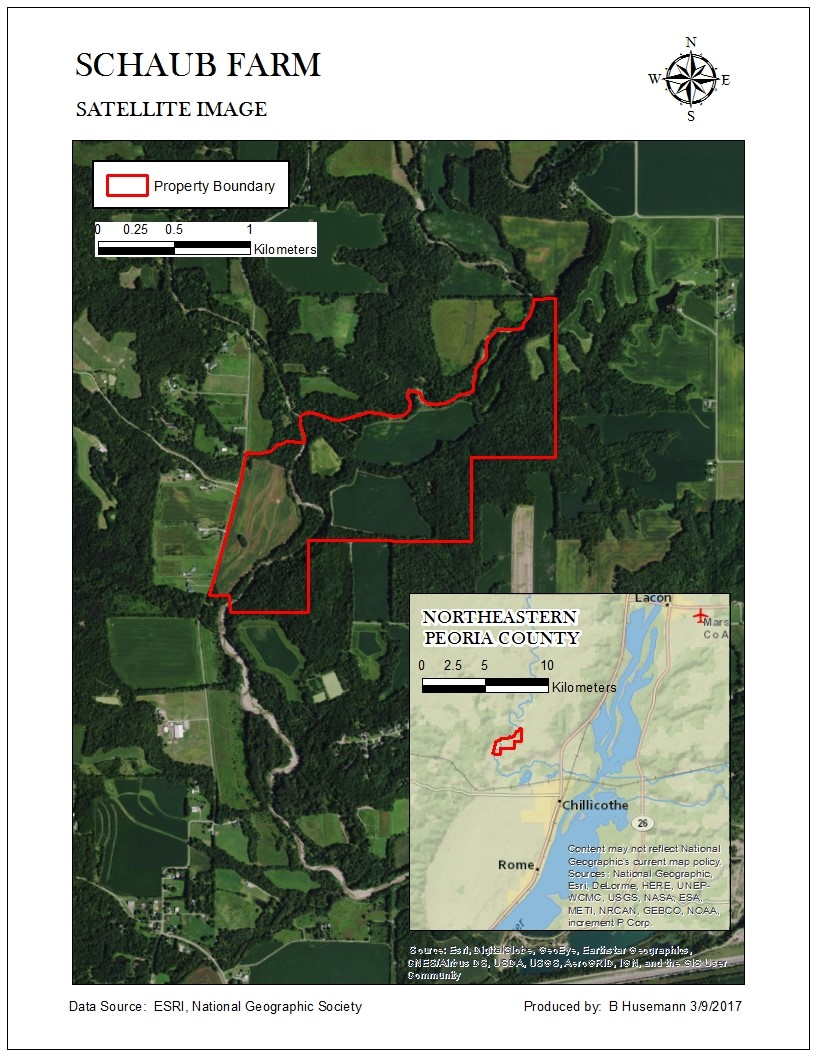
\includegraphics[width=\linewidth]{Husemann_Figure_01}
	\caption{Satellite image of Schaub farm
		{\normalfont\scriptsize \\ \copyright\ by Bradley Husemann
			%\shortauthor
			% or NAME OF COPYRIGHT HOLDER
	}}
	\label{fig:Husemann_Figure_01}
\end{figure}

\IJSRAsection{Environmental and Cultural Background}

The study area is located on the Schaub family farm, a tract of approximately 300 acres in Central Illinois. The Schaub farm is a combination of agricultural land, Conservation Reserve Program (CRP) prairie grass, and secondary growth forest (see \cref{Husemann_Figure_01}). It is split between Hallock and Chillicothe Townships in northeastern Peoria County, Illinois; the nearest town is North Hampton, a small, unincorporated community located in Hallock Township. The larger town of Chillicothe lies approximately three kilometers to the south, and the Illinois River lies roughly three kilometers to the east.

No prior archaeological study had ever taken place on the property; however, landowner Tony Schaub offered some anecdotal accounts of projectile point/knives found on the farm. These artifacts were no longer in his possession, so they could not be examined; furthermore, they would have had no clear provenience.

\IJSRAsubsection{Environmental Background}

The farm is located within the vicinity of several ecological regions, or “ecoregions,” as designated by the Environmental Protection Agency (EPA). It lies entirely within an ecoregion known as the River Hills, which consists of the steep bluffs that rise above the Illinois River, dissected in many places by narrow creeks (\cite{epa}). This ecoregion could be very suitable for early human habitation, given the combination of high ground and easy access to running water (see \cref{Husemann_Figure_02}).

%FIGURE 2: Map of ecological regions near Schaub farm
\begin{figure}[!htb]
	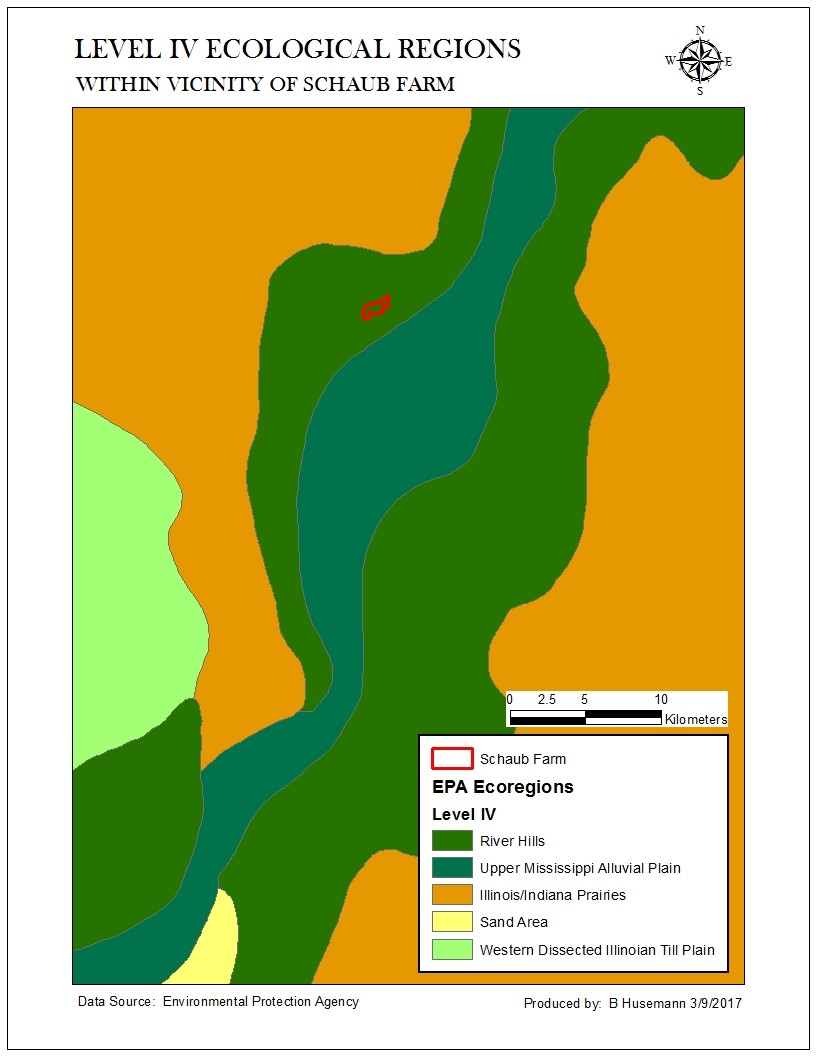
\includegraphics[width=\linewidth]{Husemann_Figure_02}
	\caption{Map of ecological regions near Schaub farm 
		{\normalfont\scriptsize \\ \copyright\ by Bradley Husemann
			%\shortauthor
			% or NAME OF COPYRIGHT HOLDER
	}}
	\label{fig:Husemann_Figure_02}
\end{figure}

The current terrain of the Schaub farm can be divided into upland terraces and lowland floodplains. On the map below (\cref{Husemann_Figure_03}), the floodplains are identified as “frequently flooded” soil types.

%FIGURE 3: Map of soil types within Schaub farm
\begin{figure}[!htb]
	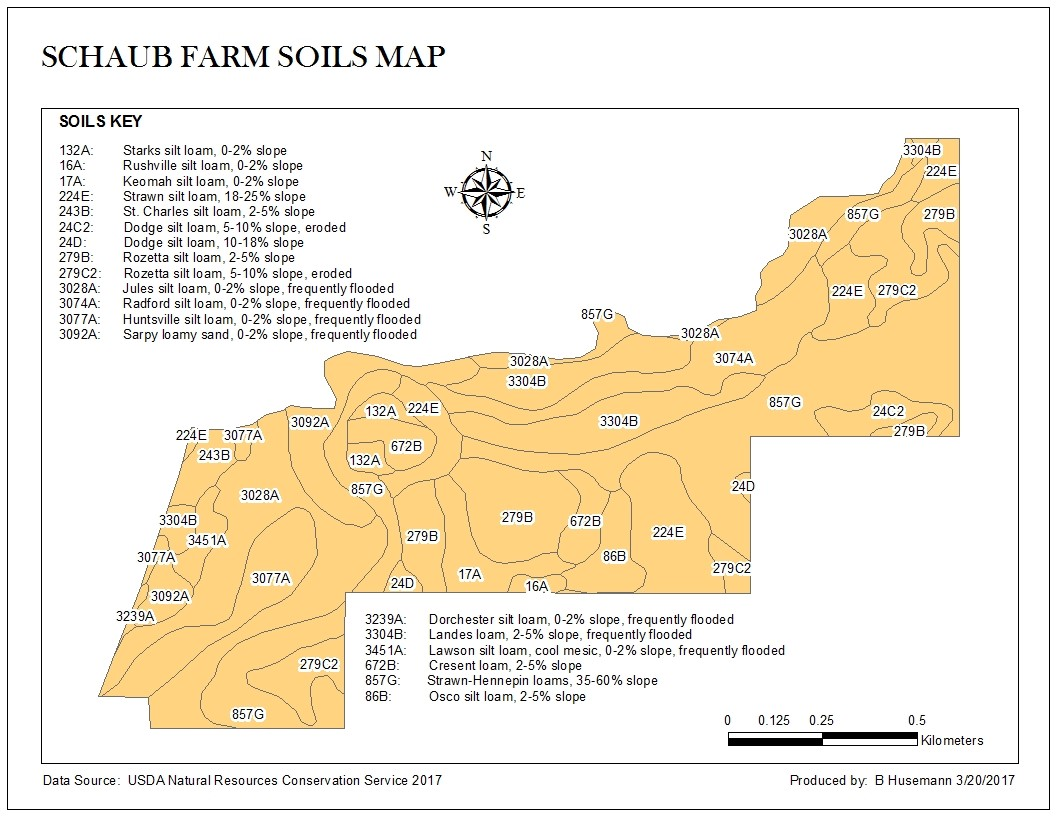
\includegraphics[width=\linewidth]{Husemann_Figure_03}
	\caption{Map of soil types within Schaub farm 
		{\normalfont\scriptsize \\ \copyright\ by Bradley Husemann
			%\shortauthor
			% or NAME OF COPYRIGHT HOLDER
	}}
	\label{fig:Husemann_Figure_03}
\end{figure}

The formation of the upland areas was influenced by glacial activity during the Pleistocene Epoch. The most recent glaciation was the Wisconsin Glacial Episode, which affected what is now Northern Illinois from approximately 23,000 to 11,500\BCE, though the glaciation lasted longer in other parts of North America (\cite{ehlers_2004}). During this time, the Laurentide Ice Sheet covered much of Northern Illinois, including what is now the Schaub farm. As the ice sheet receded, meltwaters from the glacier carried silt particles out onto the lower plains, and the wind picked up these particles and deposited them on upland areas, as periglacial loess. Because this accumulation of loess mainly occurred during the glacial episodes, there has probably been very little new deposition on these upland landforms since the end of the Pleistocene (\cite{carroll_1970}). Without any deposition of new sediment to bury cultural remains, any artifacts left on these upland areas since 11,500\BCE would probably be located at or near the ground surface, without any chronological stratification.

Because the lowland areas are prone to flooding, much of the sediment there is likely alluvial in origin, and its deposition could possibly be much more recent than that of the upland loess. If this were so, then some cultural remains could be buried deep beneath the recent sediment, leading to a possible chronological stratification of artifacts.

\IJSRAsubsection{Cultural Background}

The earliest inhabitants of Central Illinois were prehistoric Native Americans. Before the arrival of Europeans, the indigenous people of eastern North America (the “Eastern Woodlands”) underwent four major cultural phases (the dates of which are very subjective, and vary by region):

\begin{itemize}
	\item Paleoindian Period (first arrivals-8000\BCE)
	\item Archaic Period (8000-1000\BCE)
	\item Woodland Period (1000 BCE-700\CE)
	\item Mississippian Period (700-1700\CE)
\end{itemize}

The basic chronology of the Eastern Woodlands is as follows: the continent’s first inhabitants (the “Paleoindians”) were hunter-gatherers. Their descendants during the Archaic Period continued to live primarily as hunter-gatherers, but they made new technological innovations, such as the creation of ground-stone artifacts, and projectile point/knives with notched or stemmed bases. Later, during the Woodland Period, the people of the Eastern Woodlands began to develop agriculture, particularly the cultivation of maize, but still relied heavily on hunting and gathering. They also developed the use of pottery. Finally, during the Mississippian Period, Native Americans in the area depended heavily on maize, and lived in settlements built around earthen mound complexes. However, this general chronology is vastly oversimplified, and there are many regional exceptions (\cite{gibbon_1998}).

The Illinois Inventory of Archaeological Sites keeps a record of all the known prehistoric sites in Illinois; however, their locations are not divulged to the general public. In fact, only a handful of prehistoric sites in Central Illinois have been made widely known. One particularly significant site is the Rench site (11P4), which is located near Mossville, Illinois, approximately eight kilometers south of the Schaub farm. An excavation at the Rench site in the early 1980s revealed charred feature stains indicative of a wigwam and a separate trench-built house, both dating to the Late Woodland or early Mississippian Period, roughly 1000 CE (\cite{mcconaughy_1985}). A little farther north, in southern Marshall County, Illinois, lies the Marshall site (11Ma269), a Native American petroglyph site of indeterminate age, discovered in 2011 (\cite{wagner_2013}).

When Europeans first documented the area in the late seventeenth century, the inhabitants of Illinois were members of the Illinois Confederacy, an alliance of tribes including the Peoria, Kaskaskia, Cahokia, and many others, all of whom used related Algonquin languages. The Illinois River valley, where the Schaub farm is located, was occupied by the Kaskaskia (\cite{murphree_2012}). Later, during the early nineteenth century, the central Illinois River valley was occupied by Kickapoo and Potawatomi settlements (\cite{wagner_2013}).

The first European settlers in the area were the French. In 1680, the French explorer Robert Cavalier Sieur de LaSalle established a short-lived stronghold known as Fort Creve Coeur along the Illinois River, east of what is now the city of Peoria. American citizens first settled at the site of Peoria (then known as Fort Clark) in 1819 (\cite{mcculloch_1902}). The first American settler in what is now Hallock Township, in northeastern Peoria County, is believed to have been Lewis Hallock, who had lived among the Native Americans as a fur trapper for many years, before building a cabin in Central Illinois in 1820. The first settler in what is now Chillicothe Township, to the east, was Mahlon Lupton, who arrived in 1829 (\cite{illinois_1880} %The History of Peoria County, Illinois, 1880
).

The first comprehensive plat map of Peoria County was drafted in 1861, by the surveyor D.B. Allen. This provides the first detailed map of the land currently occupied by the Schaub farm. Two early landowners, T. Baldwin and E.L. Burnett, owned structures on their respective parcels, and both of these structures appear to be in or near the current boundaries of the Schaub farm. In 1861, Senachwine Creek was drawn flowing to the west of the Baldwin house, but since then, it has shifted eastwards considerably. It is likely that the creek undercut and obliterated the Baldwin house (\cite{allen_1861}).

In the map below (\cref{fig:Husemann_Figure_04}), the modern boundaries of the Schaub farm can be seen superimposed against the 1861 plat:

%FIGURE 4: 1861 plat map
\begin{figure}[!htb]
	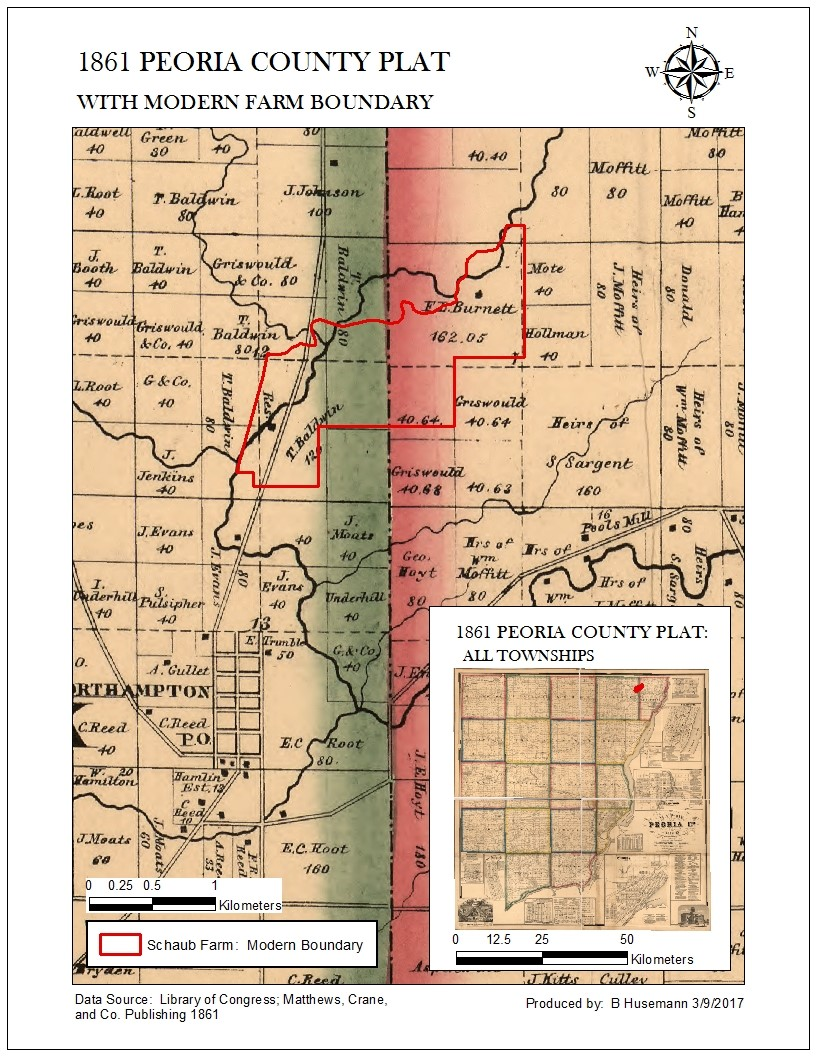
\includegraphics[width=\linewidth]{Husemann_Figure_04}
	\caption{1861 plat map 
		{\normalfont\scriptsize \\ \copyright\ by Bradley Husemann
			%\shortauthor
			% or NAME OF COPYRIGHT HOLDER
	}}
	\label{fig:Husemann_Figure_04}
\end{figure}


Another plat map of Peoria County was drawn in 1873, by the surveyor A.T. Andreas. A portion of Andreas’ atlas, featuring Chillicothe Township, is shown below (\cref{fig:Husemann_Figure_05}). According to the atlas, the area that now comprises the Schaub farm contained two structures in 1873 (on the eastern side of the township boundary). One structure belonged to F.S. Wilmot, who owned a large, heavily wooded parcel. Roughly half a kilometer to the southwest, there was another structure on a smaller parcel owned by S.M. Murry, or possibly Murray (\cite{andreas_1873}).

%FIGURE 5: 1873 plat map
\begin{figure}[!htb]
	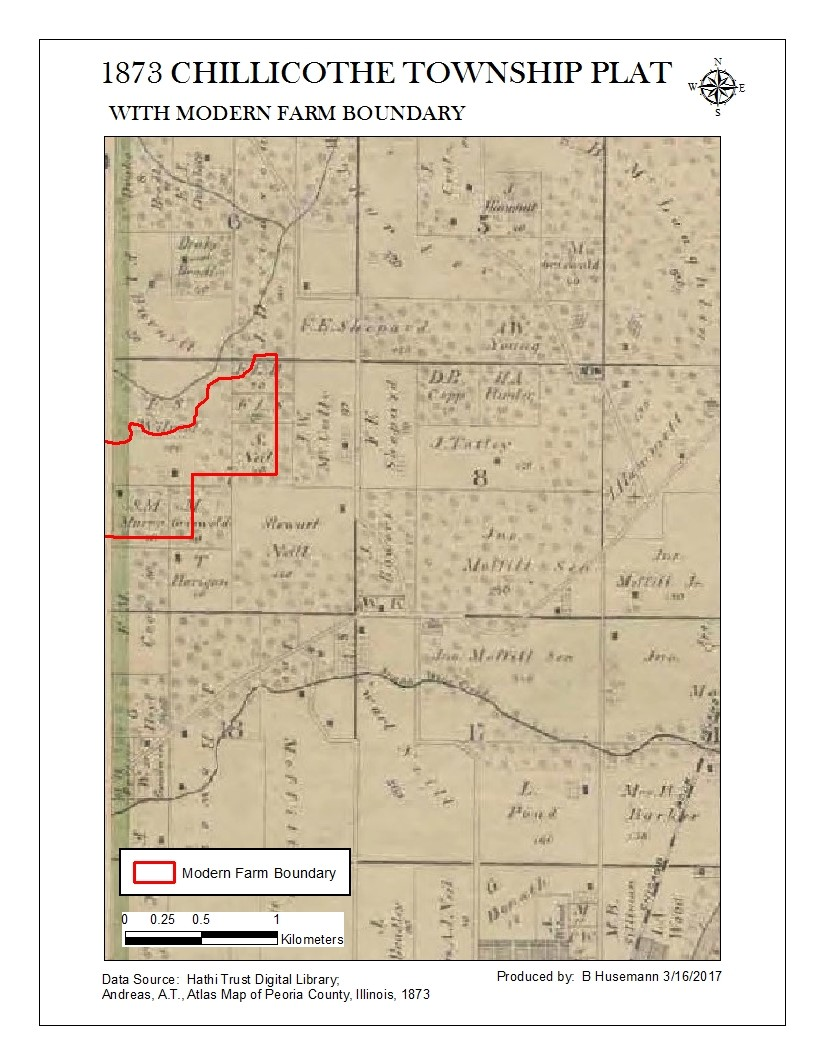
\includegraphics[width=\linewidth]{Husemann_Figure_05}
	\caption{1873 plat map 
		{\normalfont\scriptsize \\ \copyright\ by Bradley Husemann
			%\shortauthor
			% or NAME OF COPYRIGHT HOLDER
	}}
	\label{fig:Husemann_Figure_05}
\end{figure}
 
One notable feature of the Schaub farm’s history is that it is located near the route once taken by the Peoria and Galena Coach Road, one of Illinois’ first official state roads. In 1833, the state of Illinois commissioned the surveyor Levi Warren to lay out an official road from Peoria to Galena, Illinois. North Hampton Road, a modern, paved thoroughfare in Hallock Township, is believed to follow roughly the same route as this early coach road (\cite{illinois} %Illinois General Assembly
). 
North Hampton Road lies directly adjacent the Schaubs’ property, and it is likely that the early coach road passed near, or through, the land that now comprises the farm (see Figure  \cref{fig:Husemann_Figure_06}). Even though the farm is currently located in a remote and sparsely populated location, at one time, it was close to one of Illinois’ major byways, which could increase the likelihood of finding historic sites.

%FIGURE 6: Map of early trail and coach road from Peoria to Galena, Illinois
\begin{figure}[!htb]
	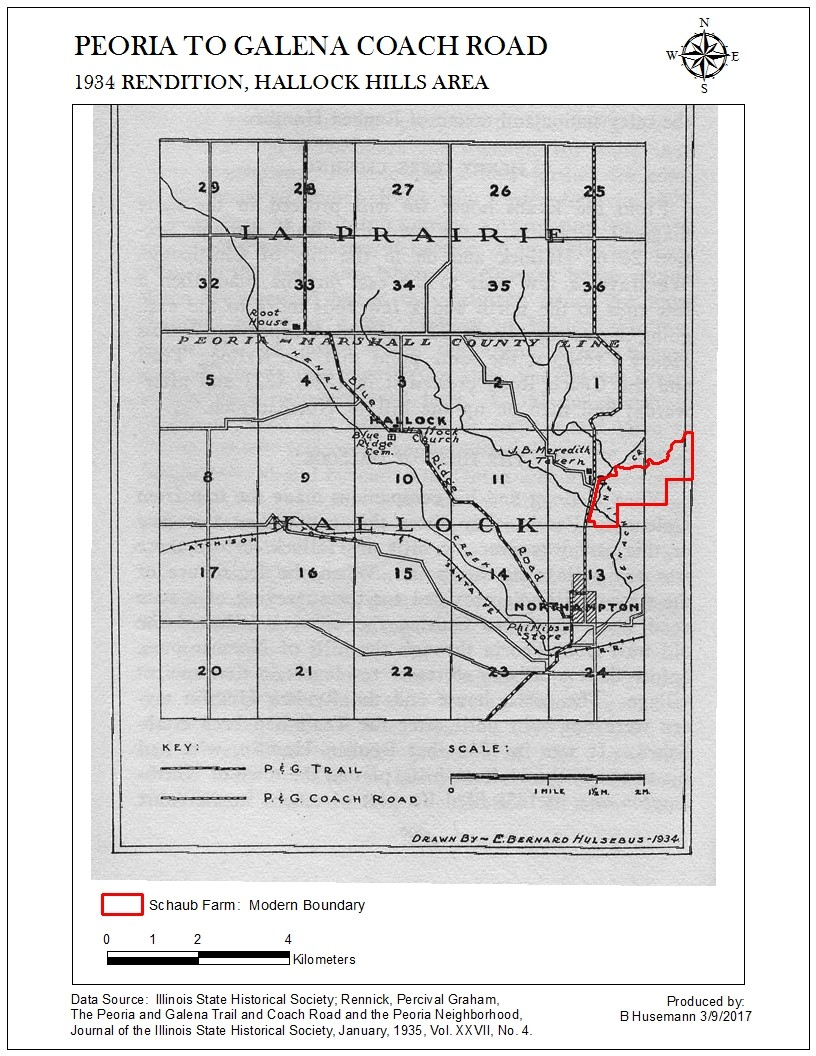
\includegraphics[width=\linewidth]{Husemann_Figure_06}
	\caption{Map of early trail and coach road from Peoria to Galena, Illinois 
		{\normalfont\scriptsize \\ \copyright\ by Bradley Husemann
			%\shortauthor
			% or NAME OF COPYRIGHT HOLDER
	}}
	\label{fig:Husemann_Figure_06}
\end{figure}

\IJSRAsection{Methods}

The survey was conducted in accordance with the regulations established by the Illinois Historic Preservation Agency (IHPA) for Section 106 compliance surveys in Illinois. Artifacts more than 50 years old were recorded, but clearly modern artifacts were ignored. 

Two survey methods were used in the field: shovel testing and pedestrian survey. The real world coordinates of every shovel test and surface find were recorded in TerraSync, using either a Trimble GeoXT or Trimble GeoXH receiver. ArcGIS was used to draft maps of the findings within the survey area.

Pedestrian survey was conducted at regular five-meter intervals in tilled agricultural fields with more than 40 percent surface visibility. It was also conducted in other areas where the ground had been mechanically disturbed.
Shovel testing was implemented in areas with less than 40 percent surface visibility, such as in wooded areas where the surface was overgrown by vegetation, and areas of no visible surface disturbance. Shovel testing was not implemented on steep slopes, drainage areas, or areas of wetland vegetation, regardless of the surface visibility (due to contextual issues and ecological sensitivity ). Additionally, if artifacts were identified in the pedestrian survey, at least one shovel test was excavated in the immediate area in order to document the stratigraphy. 
40x40 centimeter test pits were conducted at 15-meter intervals along the natural contours of the land. Pits were excavated at least ten centimeters into the subsoil (B horizon) and sieved through 1/4 inch hardware cloth. The stratigraphy of each shovel test was documented by color and texture, using Munsell color codes and USDA textural classes. The individual strata were measured by depth, and classified by pedologic horizon (i.e., Ap horizon, Bt horizon, etc.).

In some places, positive shovel tests were flanked with radial tests, in order to more closely define the site’s boundary. Radial shovel tests were placed at five-meter intervals, with the goal of producing two consecutive negative tests. The first radial would be placed ten meters from the primary positive test, and if negative, another radial would be placed at five meters from the primary. If the ten-meter radial was positive, another radial would be placed at 15 meters.

While delineating the site(s), any artifacts that were more than 100 meters apart, with no other artifacts between them, would be considered to belong to separate sites. Any artifacts within 100 meters of one another would be considered part of the same site, regardless of temporal or cultural affiliation. Any site that contained both prehistoric and historic remains, either overlapping each other or in close proximity to one other, would be characterized as “multi-component.”

It was not feasible to methodically survey all 300 acres of the Schaub farm, so a smaller research area was defined. The actual survey area was restricted to 78 acres within the middle of the farm. The survey area encompassed two frequently tilled agricultural fields, as well as a large patch of woodland. One of the agricultural fields occupies an upland terrace, overlooking Senachwine Creek to the west. Directly to the east, across a steep ravine, lies another upland terrace, this one heavily wooded.  Both terraces overlook a floodplain to the north, formed by alluvial sediment from the Senachwine’s overflow. This floodplain is also occupied by an agricultural field.  The full survey area can be seen outlined below (\cref{fig:Husemann_Figure_07}).

%Fig 7 is in multiple parts

\IJSRAsection{Survey Results}

Over the course of the survey, a large, previously unknown archaeological site was discovered and documented, Site 11P852. This site contains an extensive prehistoric component that overlaps or comes in close proximity to two distinct historic components (\cref{fig:Husemann_Figure_10}). It is almost certain that the site extends well beyond the arbitrary boundaries of the survey area, as some artifacts were found far outside the survey area, but they were not recorded. Thus, the site cannot be said to have been fully delineated (though its boundaries within the survey area were defined).

%FIGURE 10: Site 11P852, within survey area
\begin{figure}[!p]
	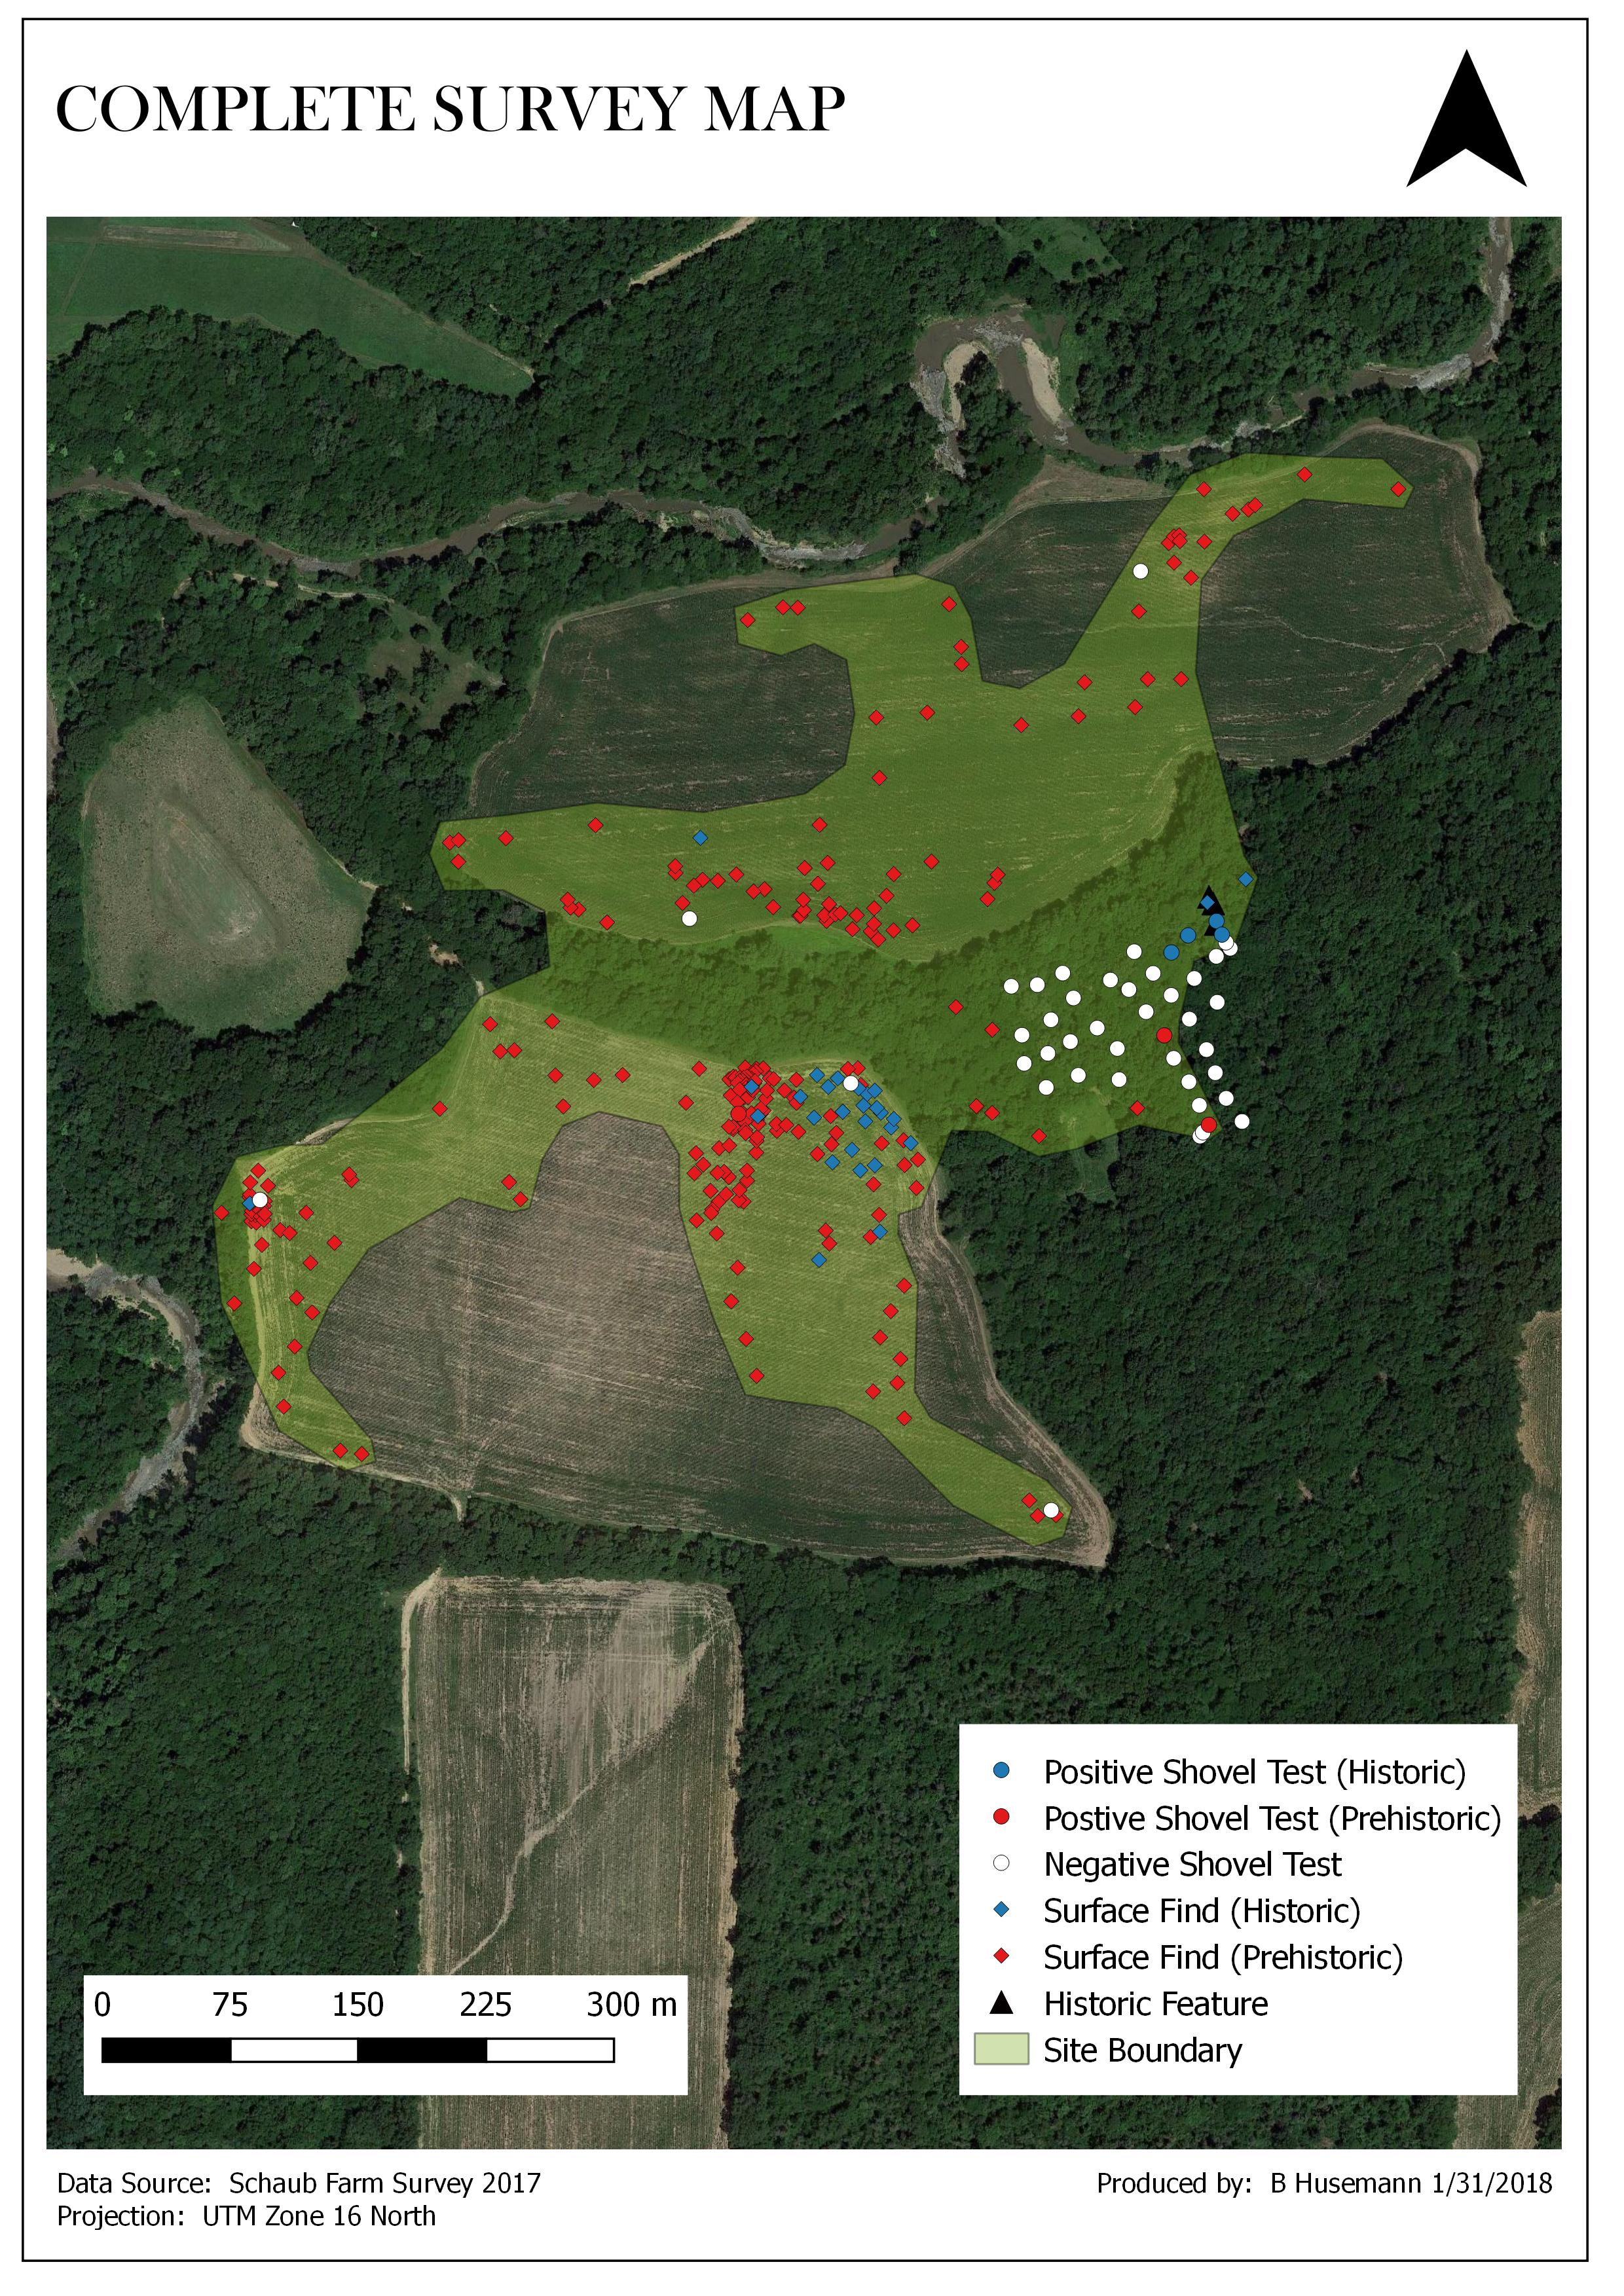
\includegraphics[width=\linewidth]{Husemann_Figure_10}
	\caption{Site 11P852, within survey area 
		{\normalfont\scriptsize \\ \copyright\ by Bradley Husemann
			%\shortauthor
			% or NAME OF COPYRIGHT HOLDER
	}}
	\label{fig:Husemann_Figure_10}
\end{figure}

\IJSRAsubsection{Prehistoric Component}


The prehistoric component is the most expansive element of the site, and extends across virtually the whole survey area (as well as beyond the survey area). The survey yielded a diverse array of prehistoric lithics; the predominant lithic material was a white chert, probably Burlington chert. The vast majority of these artifacts were flakes of lithic debitage (knapping debris), some of which display evidence of having been retouched along the edges. These artifacts were scattered across both of the upland terraces, as well as the lowland floodplain to the north, but they were mainly concentrated on a high spot along the gently undulating surface of the western terrace. Artifacts are also heavily distributed along the western and northern edges of this terrace (\cref{fig:Husemann_Figure_11}). Some flakes were even noticed on the face of a cliff overlooking Senachwine Creek, indicating that the ground has been eroded out from under them (however, due to the dangers involved, these flakes were not recovered or mapped).

%FIGURE 11: Map of prehistoric lithic scatter
\begin{figure}[!p]
	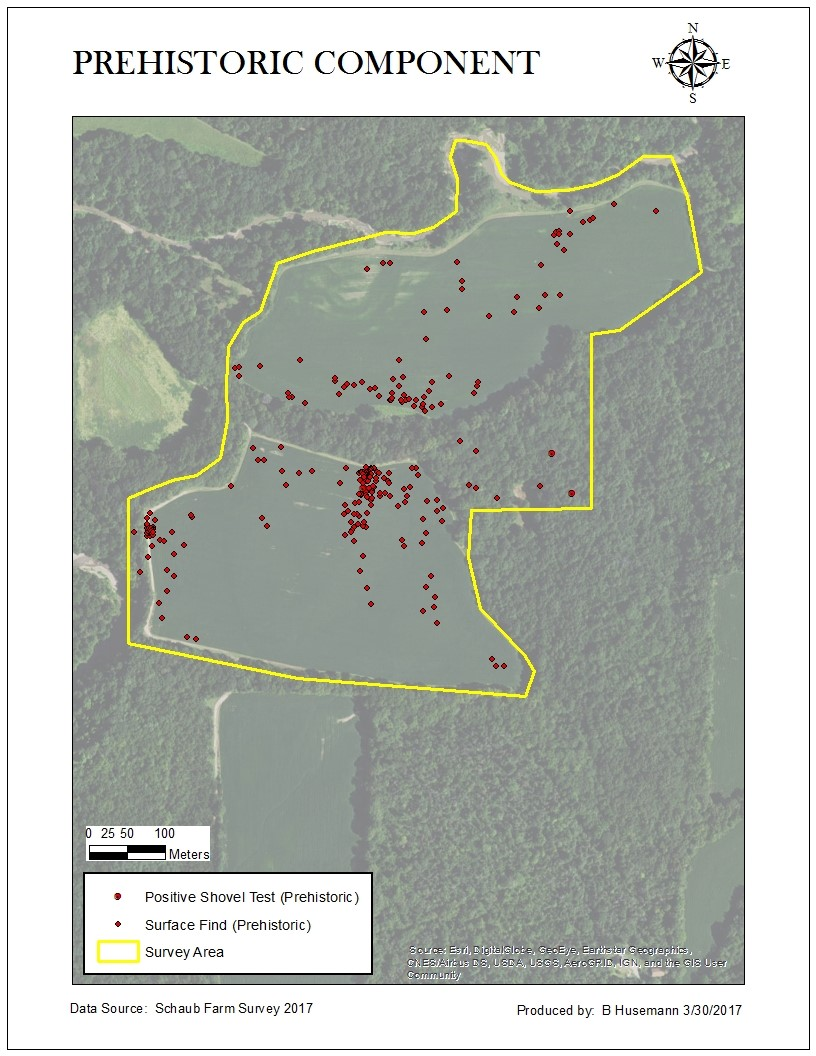
\includegraphics[width=\linewidth]{Husemann_Figure_11}
	\caption{Map of prehistoric lithic scatter
		{\normalfont\scriptsize \\ \copyright\ by Bradley Husemann
			%\shortauthor
			% or NAME OF COPYRIGHT HOLDER
	}}
	\label{fig:Husemann_Figure_11}
\end{figure}

Most of these artifacts were recovered by pedestrian survey, but a few were found in shovel tests. All of the artifacts found in shovel tests were recovered from the A horizon (topsoil), no more than 40 centimeters below the surface. Shovel tests throughout most of the site were fairly similar, with minor local differences.  A typical test revealed an Ap horizon (plow zone) extending 30-50 centimeters below the surface, ranging in color from 10YR4/3 to 10YR5/3, and ranging in texture from a silty loam to a silty clay loam.  Below the Ap horizon was a Bt horizon, ranging in color from 10YR5/4 to 10YR5/6, and ranging in texture from a silty loam to a silty clay.

312 prehistoric artifacts were recovered, including:

\begin{itemize}
	\item 4 projectile point/knives
	\item 3 broken point tips
	\item 1 drill tip
	\item 1 celt (polished stone adze)
	\item 1 bifacial scraper
	\item 3 biface fragments
	\item 1 possible fire-cracked rock (FCR)
	\item 10 cores or core fragments
	\item 288 fragments of lithic debitage (including retouched flakes)
\end{itemize}

The four projectile point/knives are intact enough to be diagnostic (\cref{fig:Husemann_Figure_12}). They indicate that the site was occupied by Native Americans over several thousand years, beginning in the Early Archaic Period (8000-6000\BCE). These typologies are tentative at best, however. 

%FIGURE 12: Diagnostic Projectile Point/Knives
\begin{figure}[!htb]
	\includegraphics[width=\linewidth]{Husemann_Figure_12}
	\caption{Diagnostic Projectile Point/Knives: a.	Kirk Corner-Notched Point, Early Archaic (8000-6000\BCE) b.	Kirk Corner-Notched Point, reversed c.	Godar Point, Middle to Late Archaic (6000-1000\BCE) d.	Godar Point, reversed e.	Osceola Point, Late Archaic to Early Woodland (3000 BCE-1\CE) f.	Osceola Point, reversed g.	Apple Blossom Point, Late Archaic to Early Woodland (3000\BCE-1\CE) h.	Apple Blossom Point, reversed
		{\normalfont\scriptsize \\ \copyright\ by Bradley Husemann
			%\shortauthor
			% or NAME OF COPYRIGHT HOLDER
	}}
	\label{fig:Husemann_Figure_12}
\end{figure}

The survey also recovered several tools or tool fragments that were not strictly diagnostic (see \cref{fig:Husemann_Figure_13}).

%FIGURE 13: Not Diagnostic Projectile Point/Knives
\begin{figure}[!htb]
	\includegraphics[width=\linewidth]{Husemann_Figure_13}
	\caption{Non- Diagnostic Tools of Tool Fragments\\
  a.	Celt \\
  b.	Celt, with cutting edge shown\\ 
  c.	Biface fragment \\
  d.	Biface fragment, reversed \\
  e.	Drill tip \\
  f.	Broken point tip
		%\shortauthor
		% or NAME OF COPYRIGHT HOLDER
}
\label{fig:Husemann_Figure_13}
\end{figure}

The map below (\cref{fig:Husemann_Figure_14}) shows the location where each projectile point/knife was recovered.

%FIGURE 14: Map of projectile point/knife locations
\begin{figure}[!htb]
	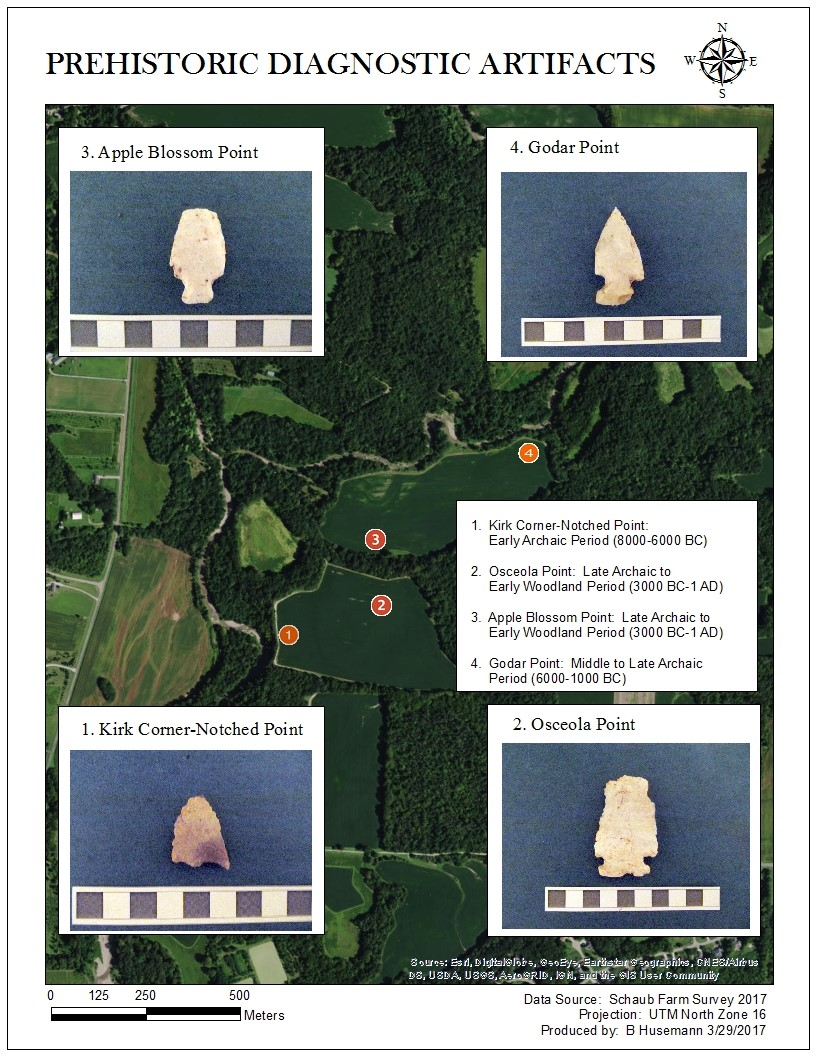
\includegraphics[width=\linewidth]{Husemann_Figure_14}
	\caption{Map of projectile point/knife locations
	%\shortauthor
	% or NAME OF COPYRIGHT HOLDER
}}
\label{fig:Husemann_Figure_14}
\end{figure}

\IJSRAsubsection{Historic Components}

Site 11P852 also includes two separate historic components, both of which correspond to houses shown on Andreas’ 1873 county plat (\cref{fig:Husemann_Figure_05}). The western historic component is a scatter of historic artifacts in a tilled field, including whiteware, vessel glass, and salt-glazed stoneware. Whiteware is a type of ceramic dishware with a white glaze, commonly used during the nineteenth and early twentieth centuries (though still made today). Salt-glazed stoneware is another, generally thicker ceramic, often used to make storage vessels; it was widely used in the nineteenth century, but still remained in use into the twentieth century. This western component contains no apparent features or structural remains, except for fragments of window glass. None of the artifacts here are diagnostic. This scatter corresponds to the location of a house on the parcel belonging to S.M. Murry (possibly Murray) on the 1873 atlas.

The eastern historic component is located on a wooded terrace overlooking the floodplain to the north. It includes three historic features, including a cellar pit, a cistern (tank for collecting rainwater), and a small pit of indeterminate usage. The cistern contains a relatively intact brick vault, with an agricultural harrow hanging into it. In the surrounding woods, there are several surface artifacts, including bricks, glass, and ceramic dishware. Shovel testing also yielded seven artifacts, including bricks, whiteware, vessel glass, and a square-cut nail; the nail most likely dates to the nineteenth century. All of these artifacts were found either within the topsoil (A horizon) or within a mottled layer of fill dirt near the features (the fill dirt was a sandy loam, 10YR5/2 mottled with 10YR5/6). In addition to the intact features, this component yielded a number of potentially diagnostic artifacts, including a sherd of ironstone dishware manufactured by J. \& G. Meakin between 1890 and 1907, and an amethyst bottle that had been decolorized with manganese dioxide, probably before the First World War. The survey also yielded a sherd of decorated salt-glazed stoneware, and a fragment of decorated blue vessel glass, which have not yet been typed. This component roughly corresponds to the location of a house that belonged to F.S. Wilmot, according to the 1873 atlas.

%FIGURE 15
\begin{figure}[!htb]
	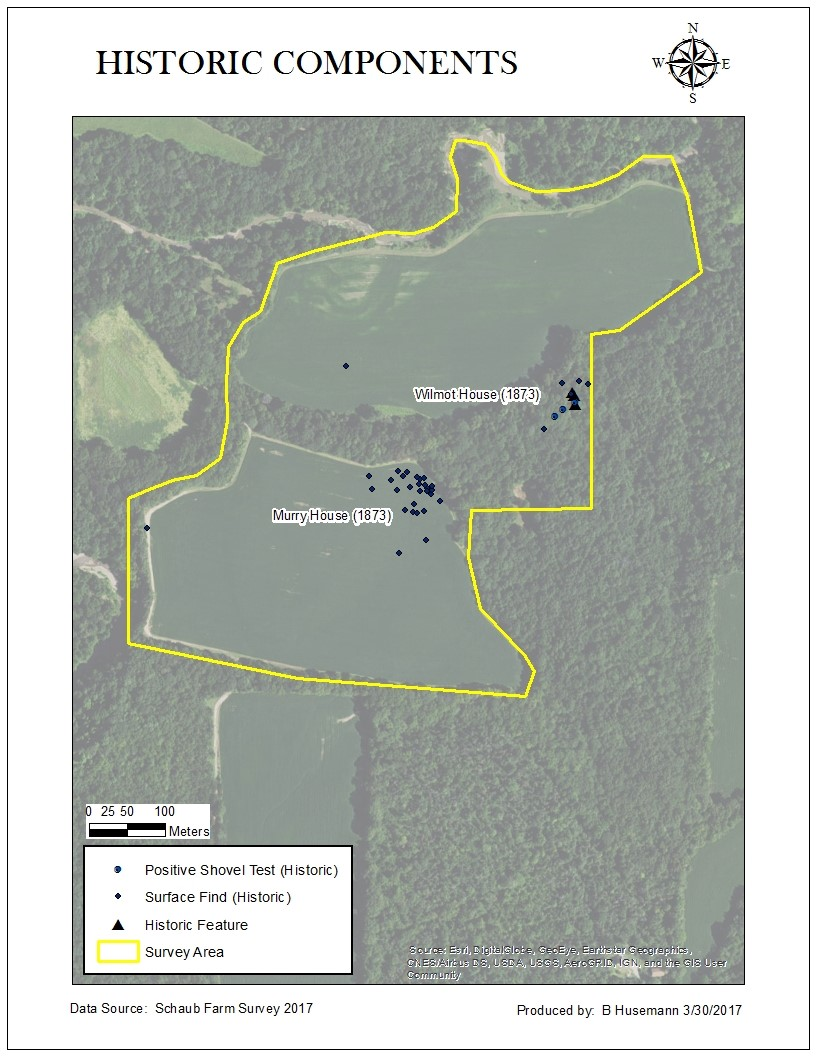
\includegraphics[width=\linewidth]{Husemann_Figure_15}
	\caption{Map of historic components 
		{\normalfont\scriptsize \\ \copyright\ by 
			%\shortauthor
			% or NAME OF COPYRIGHT HOLDER
	}}
	\label{fig:Husemann_Figure_15}
\end{figure}

%FIG 16
\begin{figure}[!htb]
	\includegraphics[width=\linewidth]{Husemann_Figure_16}
	\caption{Cellar pit, Wilmot house, viewshed facing southeast, with cistern in background
		{\normalfont\scriptsize \\ \copyright\ by 
			%\shortauthor
			% or NAME OF COPYRIGHT HOLDER
	}}
	\label{fig:Husemann_Figure_16}
\end{figure}

%FIG 17
\begin{figure}[!htb]
	\includegraphics[width=\linewidth]{Husemann_Figure_17}
	\caption{Interior of brick vault cistern, Wilmot house, with collapsed agricultural machinery
		{\normalfont\scriptsize \\ \copyright\ by 
			%\shortauthor
			% or NAME OF COPYRIGHT HOLDER
	}}
	\label{fig:Husemann_Figure_17}
\end{figure}

%FIG 18
\begin{figure}[!htb]
	\includegraphics[width=\linewidth]{Husemann_Figure_18}
	\caption{Historic artifacts from Wilmot house:\\
a.	J. \& G. Meakin Ironstone Dishware, 1890-1907\\
b.	Decorated salt-glazed stoneware with maker’s mark\\
c.	Decorated vessel glass\\
d.	Square-cut nail
		{\normalfont\scriptsize \\ \copyright\ by 
			%\shortauthor
			% or NAME OF COPYRIGHT HOLDER
	}}
	\label{fig:Husemann_Figure_18}
\end{figure}

\IJSRAsection{Discussion} 

At the beginning of the survey, five specific research questions were stated. Ultimately, the survey was able to answer all five.

\begin{enumerate}
	\item What archaeological sites, if any, are located within the survey area?
\end{enumerate}

The survey located exactly one archaeological site within the 78-acre research area; the Illinois State Museum registered it as 11P852. The site boundary is fairly subjective. This survey classified any cultural resources located within 100 meters of one another as being part of the same site, but other surveyors might have used different parameters, which would have required that 11P852 be divided into multiple sites. In all likelihood, the site actually extends well beyond the survey area, so more research would be required to fully delineate the site.

\begin{enumerate}[resume]
	\item What kinds of archaeological deposits (i.e., artifacts, features), if any, are located within the survey area?
\end{enumerate}

The survey area contains both prehistoric and historic archaeological remains. Over 300 prehistoric artifacts were recovered, all of them lithics (primarily lithic debitage). Aside from the fragments of debitage, there were also four relatively intact projectile point/knives, three broken point tips, three biface fragments, a drill tip, a bifacial scraper, 10 cores or core fragments, and one ground-stone tool (a celt, or polished adze). The presence of these prehistoric artifacts supports the assumption that the River Hills ecoregion would have been a hospitable place for early humans.
The survey also yielded three historic features and several historic artifacts. The features include a cellar pit, a brick vault cistern, and a small pit of uncertain usage. The artifacts include samples of whiteware, salt-glazed stoneware, window glass, vessel glass, bricks, and one square nail. This seems to vindicate the earlier assumption that the survey area’s proximity to the Peoria and Galena Coach Road might increase the possibility of finding historic remains. Also, the 1873 county plat had alluded to the possibility of finding historic sites.

\begin{enumerate}[resume]
	\item What is the horizontal and vertical distribution of archaeological deposits within the survey area?
\end{enumerate}

Archaeological deposits were scattered across large swaths of the survey area. The prehistoric lithics were found on both of the upland terraces, as well as the lowland floodplain. Their greatest concentration was on the western terrace, particularly on a high spot along the terrace’s surface. A detailed map of their distribution can be seen in \cref{fig:Husemann_Figure_12}. It is worth noting that artifacts may seem most prevalent on the western terrace because they were more exposed, due to tillage. Were the eastern terrace not so heavily forested, more artifacts might have been seen there.

The historic artifacts and features were divided into two main concentrations, or “components.” Each of these concentrations was once the location of a house, according to the 1873 plat. One concentration was located on the western terrace, and the other on the eastern terrace, as seen in \cref{fig:Husemann_Figure_16}.

As for the vertical, or stratigraphic, distribution of artifacts, all were located either on the surface or in the topsoil (no more than 40 centimeters deep). A few were found within an artificial layer of fill, associated with the historic features. None were found in the subsoil, and there is no evidence of stratification by time period. Earlier, it was speculated that most of the artifacts found on the upland loess terraces would be concentrated at or near the surface, due to a lack of recent deposition. The survey findings vindicated this assumption. However, it was also speculated that any artifacts found on the floodplain might be buried beneath layers of alluvial sediment, leading to possible chronological stratification. The survey findings did not support this speculation. All of the artifacts found on the floodplain were located on the surface; none were buried.

\begin{enumerate}[resume]
	\item What is the approximate temporal and/or cultural affiliation of the archaeological deposits within the survey area?
\end{enumerate}

The four projectile point/knives hint at the temporal affiliation of the prehistoric remains; it appears that the site may have been occupied by Native Americans from the Early Archaic Period (8000-6000\BCE) to the Early Woodland Period (1000\BCE-1\CE). As of yet, there is no evidence of any prior or subsequent prehistoric habitation, but it is still fully possible that such evidence may surface. All that can be said with certainty is that Native Americans occupied the site over a broad period of time, beginning during a period when they would have been predominantly hunter-gatherers, and possibly extending into a period when agriculture and the use of ceramics became more widespread (though no prehistoric ceramics were found). Throughout most of this time period, the site probably would have been used as a temporary campsite by transient hunters.
The historic artifacts and features, having been left by American settlers, belong to a much narrower spectrum of time, ranging from the late nineteenth century to the early twentieth century. Historic evidence indicates that there were two houses within the survey area at least as early as 1873 (but after 1861). A sherd of ironstone dishware associated with the Wilmot house can be positively dated between 1890 and 1907. An amethyst bottle, also affiliated with the Wilmot house, was probably made prior to the First World War.

\begin{enumerate}[resume]
	\item Do any of the archaeological deposits retain enough integrity to offer meaningful data for interpretation?
\end{enumerate}

The integrity and significance of the site are mixed, depending on which portion of the site is considered. Because the site is so large, some areas are much more intact than others, and some areas are more significant than others.
The prehistoric component has already yielded four diagnostic artifacts and several tools or tool fragments, as well as over 300 other artifacts, which is a fairly significant development. It may be able to offer considerable data for interpretation, if it were to be excavated in the future. Also, the antiquity of the site, possibly dating back to the Early Archaic Period, could add to its significance. 

However, the site’s integrity has been damaged by agricultural plowing. Most of the prehistoric component has been thoroughly plowed, and the plowing has possibly displaced or damaged many artifacts, as well as destroyed any feature stains, though there may be intact portions of features below the plow zone. It is worth noting that many of the prehistoric artifacts are still concentrated on high spots in the landscape, which are likely settlement areas, indicating that these artifacts have not moved far from where they were left. These artifacts may be relatively in situ, despite the plow damage.

Erosion has also damaged the site, particularly on the western side of the terrace overlooking Senachwine Creek. The western side of the terrace is a cliff that faces the convex side of a bend in the creek, and as the creek has slowly swung eastwards over time, it has been eroding the terrace. Part of the site has already been eroded away, as evidenced by prehistoric artifacts found on the face of the cliff. It is not clear how much of the site has already been destroyed in this manner.

%FIG 19
\begin{figure}[!htb]
	\includegraphics[width=\linewidth]{Husemann_Figure_19}
	\caption{Cliff overlooking Senachwine Creek, viewshed facing south
		{\normalfont\scriptsize \\ \copyright\ by 
			%\shortauthor
			% or NAME OF COPYRIGHT HOLDER
	}}
	\label{fig:Husemann_Figure_19}
\end{figure}

The two historic components are very unequal in their integrity. The westernmost component (the Murry house) has been extensively plowed, and has no features, structural remains, or diagnostic artifacts. Very little remains intact, and it offers very little data for interpretation. However, the easternmost historic component (the Wilmot house) may be the most intact portion of the whole site. It has three intact features, in addition to multiple diagnostic artifacts. Furthermore, it does not appear to have been plowed. This component could offer significant data for interpretation, but its relatively recent age (late nineteenth century and early twentieth century) could dissuade scholarly interest.

\IJSRAsection{Conclusion}

The survey indicated that the Schaub family farm does, in fact, contain substantial archaeological remains. Only a relatively small section of the farm was surveyed, but this survey area yielded an extensive archaeological site, with a large prehistoric component and two separate historic components. The prehistoric component seems to consist entirely of lithics, including four diagnostic projectile point/knives, several other tools or tool fragments (including a celt and drill tip), and nearly 300 flakes of lithic debitage. The two historic components both seem to date to the late nineteenth or early twentieth centuries; they include fragments of window glass, vessel glass, whiteware, stoneware, and bricks, among other artifact types. One of the historic components, corresponding to the house owned by F.S. Wilmot on the 1873 county atlas, also contains three intact features (including a cellar pit and a brick vault cistern), potentially making it the most intact portion of the site.

\IJSRAseparator

\IJSRAsection{Acknowledgements}

The author would like to acknowledge the Schaub family for allowing the survey to take place on their farm; Dr. Scott Palumbo, for agreeing to supervise the project; and James Parker of HDR, Inc., for assisting in the analysis of historic artifacts and features. And a special thanks to the Starbucks at the corner of Prospect and War Memorial in Peoria, Illinois, for letting the author use their internet connection, even while covered in mud from the field.


\IJSRAclosing%<---- don’t change this!